\documentclass[12pt,aspectratio=169]{beamer}

% ====================================================
% ====================================================
% USEPACKAGES AND IMPORTS
% ====================================================
% ====================================================

\usepackage[T1]{fontenc}
\usepackage[utf8]{inputenc}
\usepackage[english]{babel}

% tables
\usepackage{tabularx}
\usepackage{colortbl}
\usepackage{multirow}
\usepackage{makecell}

% tikz and colors
\usepackage{tikz}
\usepackage{xcolor}
\usepackage{pgfplots}
\usepackage{pgfplotstable}
\usepackage{tikzsymbols}

\usetikzlibrary{calc}
\usetikzlibrary{trees}
\usetikzlibrary{patterns}
\usetikzlibrary{shadings}
\usetikzlibrary{positioning}
\usetikzlibrary{intersections}
\usepgfplotslibrary{patchplots}
\usepgfplotslibrary{fillbetween}
\usetikzlibrary{decorations.pathreplacing}

\usetikzlibrary{arrows}
\usetikzlibrary{arrows.meta}

\usetikzlibrary{shapes}
\usetikzlibrary{shapes.arrows}
\usetikzlibrary{shapes.callouts}
\usetikzlibrary{shapes.symbols}
\usetikzlibrary{shapes.geometric}

% boxes
\usepackage[many]{tcolorbox}

% math packages and fonts
\usepackage{bm}
\usepackage{ccfonts}
\usepackage{eulervm}
\usepackage{amsmath}
\usepackage{amsfonts}
\usepackage{amssymb}
\usepackage{amsthm}
\usepackage{mathtools}
\usepackage{nicefrac}
\usepackage{slashed}
\usepackage{bbold}
\usepackage{array}
\usepackage{cancel}

% algorithms and listings
\usepackage[ruled,vlined,linesnumbered]{algorithm2e}
\usepackage{listings}
\usepackage{setspace}

\tcbuselibrary{listings}
\tcbuselibrary{breakable}
\tcbuselibrary{skins}

% misc
\usepackage{soul}
\usepackage{pifont}
\usepackage{skull}
\usepackage{multicol}
\usepackage{animate}
\usepackage{hyperref}
\usepackage{wasysym}
\usepackage[absolute,overlay]{textpos}
\usepackage[hang,flushmargin]{footmisc}

% ====================================================
% ====================================================
% LAYOUT AND THEME
% ====================================================
% ====================================================

\usetheme{Copenhagen}

% color definitions
\definecolor{myblue1}{RGB}{35,119,189}
\definecolor{myblue2}{RGB}{95,179,238}
\definecolor{myblue3}{RGB}{129,168,207}
\definecolor{myblue4}{RGB}{26,89,142}

\definecolor{myred1}{RGB}{247,12,12}

% set theme colors
\setbeamercolor*{structure}{fg=myblue1,bg=blue}
\setbeamercolor*{palette primary}{use=structure,fg=white,bg=structure.fg}
\setbeamercolor*{palette secondary}{use=structure,fg=white,bg=structure.fg!75!black}
\setbeamercolor*{palette tertiary}{use=structure,fg=white,bg=structure.fg!50!black}
\setbeamercolor*{palette quaternary}{fg=black,bg=white}

\setbeamertemplate{itemize item}[circle]
\setbeamertemplate{itemize subitem}[circle]
\setbeamertemplate{itemize subsubitem}[circle]

\setbeamertemplate{enumerate item}[circle]
\setbeamertemplate{enumerate subitem}[circle]
\setbeamertemplate{enumerate subsubitem}[circle]

\setbeamercolor{itemize item}{fg=myblue1}
\setbeamercolor{itemize subitem}{fg=myblue1}
\setbeamercolor{itemize subsubitem}{fg=myblue1}

\setbeamertemplate{section in toc}[circle]
\setbeamertemplate{subsection in toc}[circle]
\setbeamerfont{subsection in toc}{size=\scriptsize}

\setbeamercolor{frametitle continuation}{fg=black}

% title graphic -- sap logo and dhbw logo
\titlegraphic{
\includegraphics[scale=0.1]{../03_img/logo_sap}\hspace*{4.75cm}~%
   	
\includegraphics[scale=0.05]{../03_img/logo_dhbw}
}

\makeatletter
% frame title
\defbeamertemplate*{frametitle}{mydefault}[1][left]
{
  	\ifbeamercolorempty[bg]{frametitle}{}{\nointerlineskip}%
  	\nointerlineskip%
 	\@tempdima=\textwidth%
  	\advance\@tempdima by\beamer@leftmargin%
  	\advance\@tempdima by\beamer@rightmargin%
  	\begin{tcolorbox}[
  		enhanced,
  		outer arc=0pt,
  		arc=0pt,
  		boxrule=0pt,
  		top=0pt,
  		bottom=0pt,
  		enlarge left by=-\beamer@leftmargin,
  		enlarge right by=-\beamer@rightmargin,
  		width=\paperwidth,
  		nobeforeafter,
  		interior style={
    			left color=myblue2,
    			right color=white
    		},
  		shadow={0mm}{-0.4mm}{0mm}{black!60,opacity=0.6},    
  		shadow={0mm}{-0.8mm}{0mm}{black!40,opacity=0.4},    
  	]
    	\usebeamerfont{frametitle}%
    	\vbox{}\vskip-1ex%
    	\if@tempswa\else\csname beamer@fte#1\endcsname\fi%
    	\insertframetitle\par%
    	{%
      		\ifx\insertframesubtitle\@empty%
      		\else%
      		{\usebeamerfont{framesubtitle}\usebeamercolor[fg]{black}\insertframesubtitle\strut\par}%
      		\fi
    	}%
    	\vskip-1ex%
    	\if@tempswa\else\vskip-.3cm\fi
  	\end{tcolorbox}%
}

% footline of a frame
\defbeamertemplate*{footline}{mysplit theme}
{%
  	\leavevmode%
  	\hbox{
		\begin{beamercolorbox}[
			wd=.5\paperwidth,ht=2.5ex,dp=1.125ex,leftskip=.3cm plus1fill,rightskip=.3cm
		]{author in head/foot}%
    			\usebeamerfont{author in head/foot}\insertshortauthor\ (\insertinstitute), \insertdate
  		\end{beamercolorbox}%
  		\begin{beamercolorbox}[
			wd=.5\paperwidth,ht=2.5ex,dp=1.125ex,leftskip=.3cm,rightskip=.3cm plus1fil
		]{title in head/foot}%
    			\usebeamerfont{title in head/foot}\insertshorttitle\hfill
    			\insertprefix-\insertframenumber/\inserttotalframenumber\hspace*{0.5em}
  		\end{beamercolorbox}}%
  	\vskip0pt%
}
\makeatother

% ====================================================
% ====================================================
% COMMANDS AND GENERAL DEFINITIONS
% ====================================================
% ====================================================

% page number prefix
\newcommand\insertprefix{}  % empty by default
\newcommand\prefix[1]{\renewcommand\insertprefix{#1}}

% math definitions
% ====================================================
\DeclareMathOperator*{\argmax}{arg\,max}
\DeclareMathOperator*{\argmin}{arg\,min}
\newcommand*\diff{\mathop{}\!\mathrm{d}}

\newcommand*{\vertbar}{\rule[-1ex]{0.5pt}{2.5ex}}
\newcommand*{\horzbar}{\rule[.5ex]{2.5ex}{0.5pt}}

% commands
% ====================================================

% highlight commands
% --------------------------------------------------------------------------------------------------------
% highlight command
\newcommand{\highlight}[1]{\textcolor{myblue1}{\textbf{#1}}}
\newcommand{\highlighttt}[1]{\textcolor{myblue1}{\texttt{#1}}}
\newcommand{\Highlight}[1]{\textcolor{myred1}{\textbf{#1}}}

% blue color boxes (with frame/without frame/without fill)
\newtcolorbox{boxBlue}{colback=myblue1!10!white,colframe=myblue4}
\newtcolorbox{boxBlueNoFrame}{colback=myblue1!10!white,colframe=myblue1!10!white}
\newtcolorbox{boxBlueNoFill}{colback=white,colframe=myblue4}

% font commands
% --------------------------------------------------------------------------------------------------------
\newcommand{\linkstyle}[1]{\underline{\smash{\texttt{#1}}}} 		% style of hyperlinks

% tikz commands
% --------------------------------------------------------------------------------------------------------

% yellow sticky note
\newcommand{\bubble}[3]{
\begin{textblock}{100}(#1, #2)
      	\begin{tikzpicture}
		\node[rectangle,draw=yellow,very thick,fill=yellow!60,align=center] at (0,0) {#3};
	\end{tikzpicture}
\end{textblock}
}

\newcommand{\floattext}[3]{
\begin{textblock}{100}(#1, #2)
      	#3
\end{textblock}
}

\newcommand{\doublecircle}[2]{
	\draw[fill=white,draw=myblue1] (#1,#2) circle (2mm);
	\draw[fill=myblue1,draw=myblue1] (#1,#2) circle (1.5mm);
}

% slide modifiers
% --------------------------------------------------------------------------------------------------------
% mark slide as optional
\newcommand{\optional}{
	\begin{textblock}{100}(0.15,0.30)
      		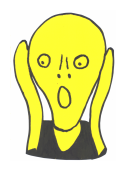
\includegraphics[scale=0.2]{../03_img/scream}
    	\end{textblock}
}

% mark slide as important
\newcommand{\important}{
	\begin{textblock}{100}(0.10,0.15)
      		
\includegraphics[scale=0.1]{../03_img/important}
    	\end{textblock}
}

% citation
% --------------------------------------------------------------------------------------------------------
% first argument in {book, online, article}
\newcommand{\literature}[5]{
	\setbeamertemplate{bibliography item}[#1]
	\bibitem{#2}
	\highlight{#3} \\
	\textcolor{darkgray}{\textit{#4}} \\
	\textcolor{black}{#5}
}
% cite content
\newcommand{\citeAuthor}[3]{\vfill\scriptsize\textcolor{lightgray}{#1 \cite{#2} #3}}

% slide architecture
% --------------------------------------------------------------------------------------------------------
% divide frame into two parts
\newcommand{\divideTwo}[4]{
	\begin{minipage}{#1\textwidth}
		#2
	\end{minipage}
	\hfill
	\begin{minipage}{#3\textwidth}
		#4
	\end{minipage}
}

% divide frame into two parts (start on top)
\newcommand{\divideTwoTop}[4]{
	\begin{minipage}[t]{#1\textwidth}
		#2
	\end{minipage}
	\hfill
	\begin{minipage}[t]{#3\textwidth}
		#4
	\end{minipage}
}

% special pages
% --------------------------------------------------------------------------------------------------------
% title page
\newcommand{\maketitlepage}{
	{
		\beamertemplatenavigationsymbolsempty
		\usebackgroundtemplate{%
			\tikz[overlay,remember picture] \node[opacity=0.2, at=(current page.center)] {
  				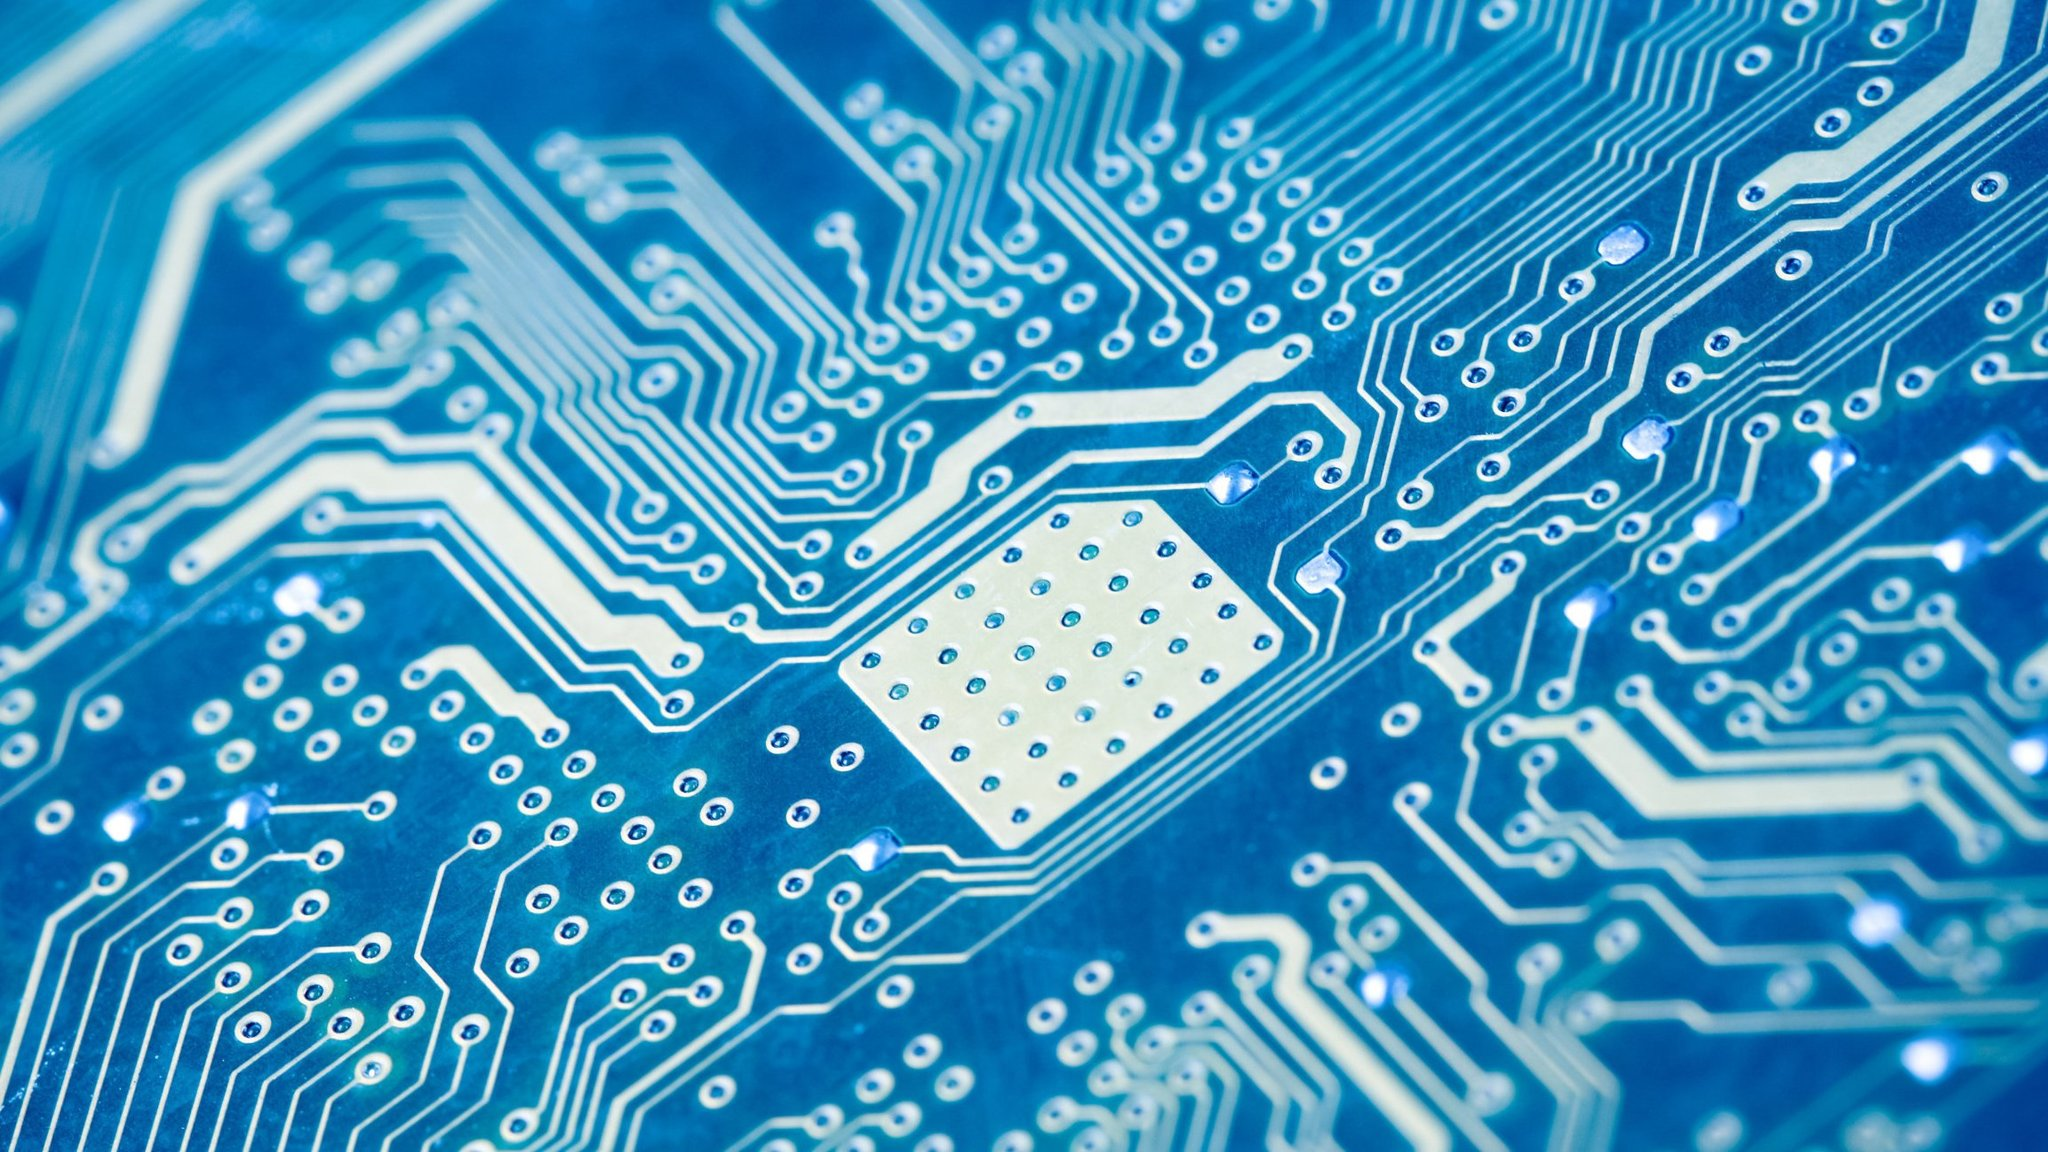
\includegraphics[height=\paperheight,width=\paperwidth]{../03_img/processor.jpg}
			};
		}
		\begin{frame}[plain]
			\vspace*{0.75cm}
			\maketitle
			\vfill
			\begin{center}
				\footnotesize Find all slides on \href{https://github.com/DaWe1992/Applied_ML_Fundamentals}{\linkstyle{GitHub}}
			\end{center}
		\end{frame}
	}
}

% divider page
\newcommand{\makedivider}[1]{
	{
		\beamertemplatenavigationsymbolsempty
		\usebackgroundtemplate{%
			\tikz[overlay,remember picture] \node[opacity=0.2, at=(current page.center)] {
  				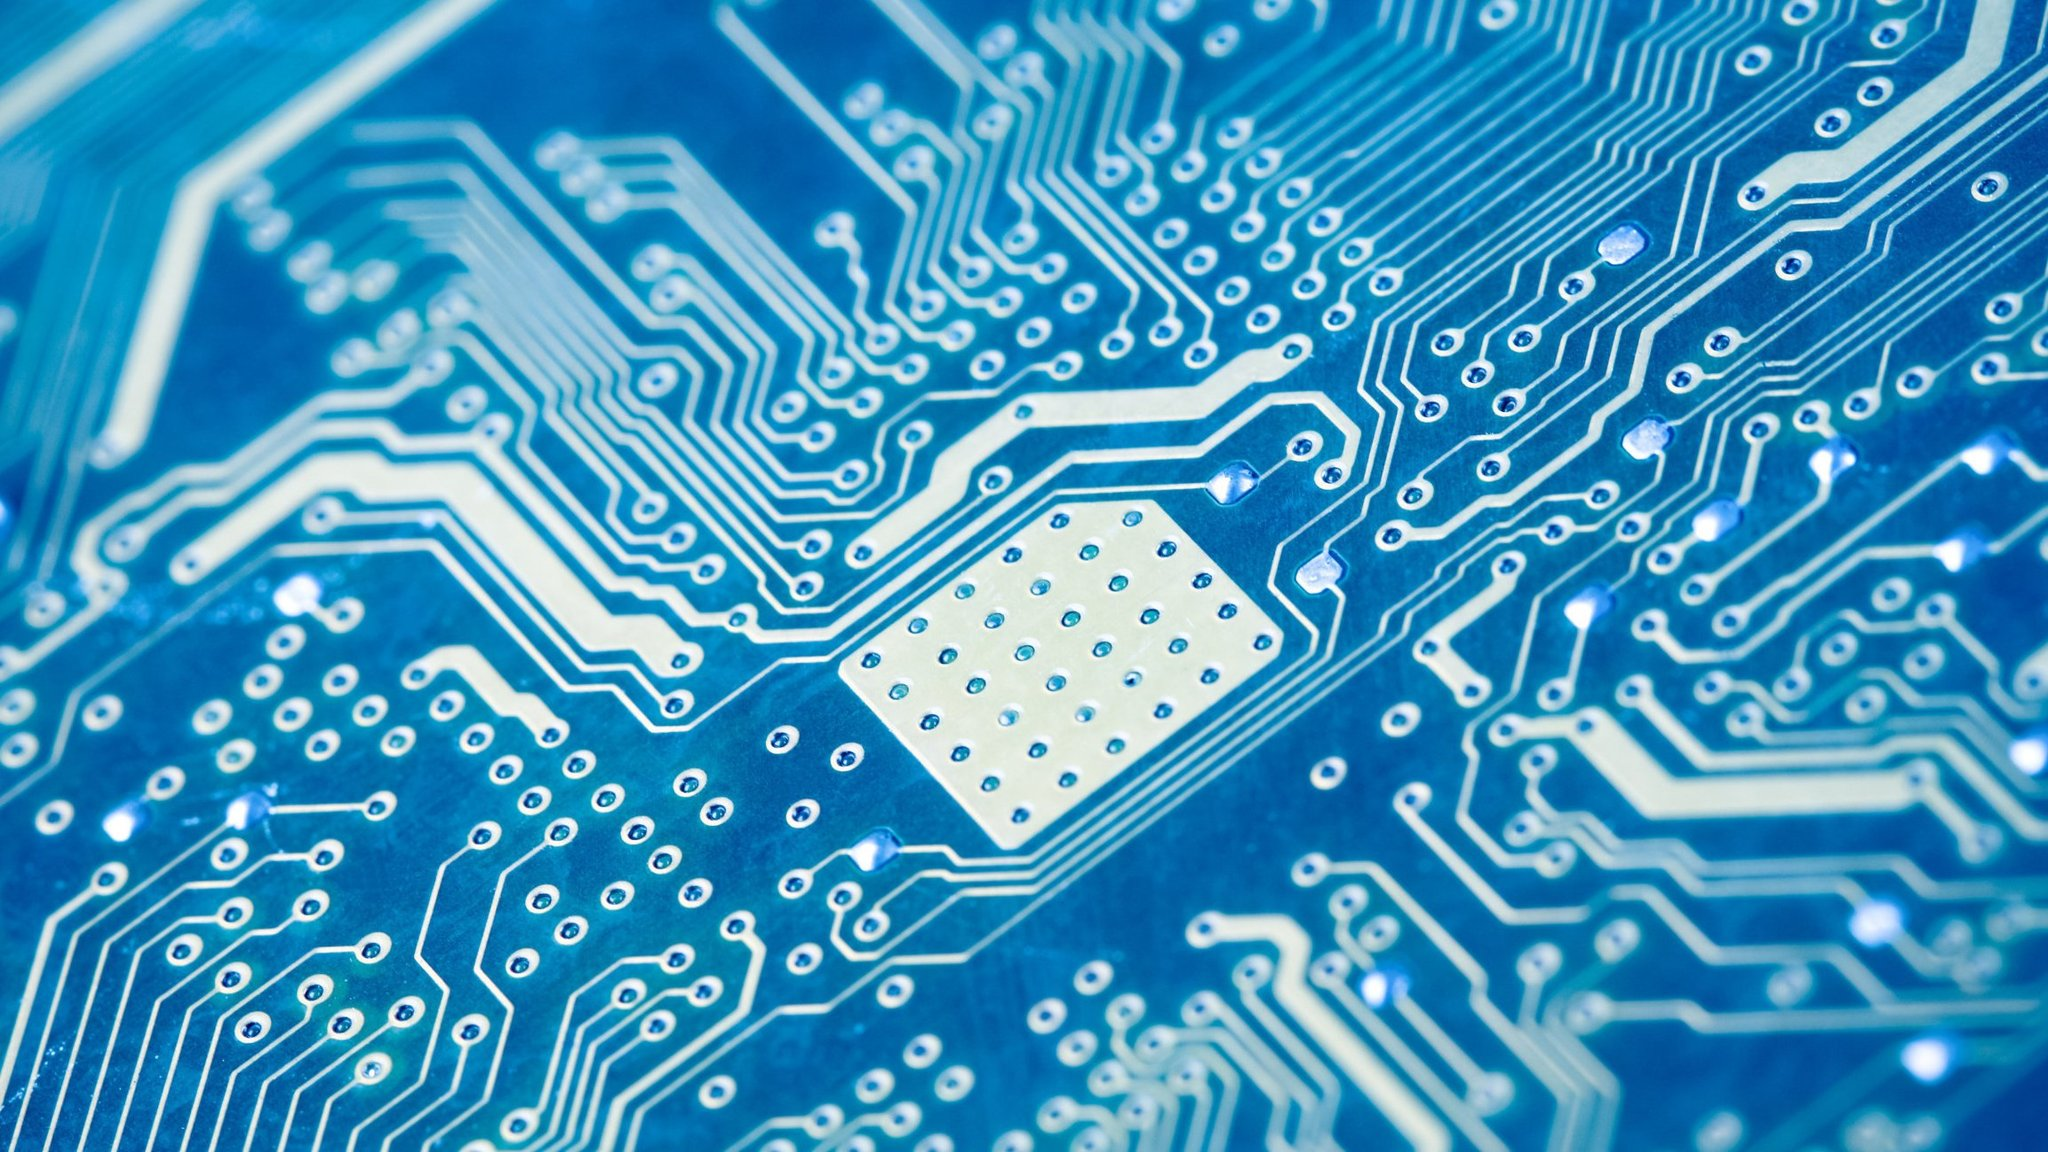
\includegraphics[height=\paperheight,width=\paperwidth]{../03_img/processor.jpg}
			};
		}
		\begin{frame}[plain]
			\vfill
			\begin{boxBlue}
				\centering
				\textbf{Section:} \\
				\large \highlight{#1}
			\end{boxBlue}
			\vfill
			\centering
			
\includegraphics[scale=0.05]{../03_img/logo_dhbw.png}
			\vfill
		\end{frame}
	}
}

% overview page
\newcommand{\makeoverview}[1]{
	\begin{frame}{Lecture Overview}{}
		\begin{tabbing}
			\hspace*{3.5cm}\= \kill
			\ifnum #1=1 \highlight{\textbf{Unit I:}} \else \textbf{Unit I:} \fi
			\> \ifnum #1=1 \highlight{Machine Learning Introduction} \else Machine Learning Introduction \fi \\
		\end{tabbing}
	\end{frame}
}

% thank you page
\newcommand{\makethanks}{
	{\beamertemplatenavigationsymbolsempty
	\begin{frame}[plain]
		\vfill
		\begin{boxBlue}
			\centering
			\Large \highlight{Thank you very much for the attention!}
		\end{boxBlue}
		
		\vfill\footnotesize
		\begin{tabbing}
			\hspace*{1.5cm}\= \kill
			\highlight{Topic:} 	\> \inserttitle \\
			\highlight{Date:} 	\> \insertdate
		\end{tabbing}
		
		\vfill
		\highlight{Contact:} \\
		\insertauthor\ (D062271) \\
		\insertinstitute \\
		\href{mailto:daniel.wehner@sap.com}{\linkstyle{daniel.wehner@sap.com}}
		
		\vfill\normalsize
		\begin{center}
			\large\highlight{Do you have any questions?}
		\end{center}
		\vfill
	\end{frame}}
}

% global pfgplots settings
% --------------------------------------------------------------------------------------------------------
\pgfplotsset{
	% allow filtering of data for pgfplots
	discard if/.style 2 args={
        		x filter/.code={
            		\edef\tempa{\thisrow{#1}}
            		\edef\tempb{#2}
            		\ifx\tempa\tempb
                		\def\pgfmathresult{inf}
            		\fi
        		}
    	},
    	discard if not/.style 2 args={
        		x filter/.code={
            		\edef\tempa{\thisrow{#1}}
            		\edef\tempb{#2}
            		\ifx\tempa\tempb
            		\else
                		\def\pgfmathresult{inf}
            		\fi
        		}
    	}
}


% ====================================================
% ====================================================
% PRESENTATION DATA
% ====================================================
% ====================================================

\title[Machine Learning Introduction]{*** Applied Machine Learning Fundamentals *** Machine Learning Introduction}
\institute{SAP\,SE}
\author{M.\,Sc. Daniel Wehner}
\date{Winter term 2019/2020}
\prefix{INTRO}

% ====================================================
% ====================================================
% BEGIN OF DOCUMENT
% ====================================================
% ====================================================

\begin{document}

% Title frame
%______________________________________________________________________
\maketitlepage


% Lecture Overview
%______________________________________________________________________
\begin{frame}{Lecture Overview}{}
	\makeoverview{1}
\end{frame}


% Agenda
%______________________________________________________________________
\begin{frame}{Agenda for this Unit}
	\begin{multicols}{2}
		\tableofcontents
	\end{multicols}
\end{frame}


% Section: Introduction
%______________________________________________________________________
\section{Introduction}
\makedivider{Introduction}

% Subsection: Motivation
% --------------------------------------------------------------------------------------------------------
\subsection{Motivation}

% Why Machine Learning?
\begin{frame}{Why Machine Learning?}{}
	\begin{itemize}
		\item \textit{`We are drowning in information and starving for knowledge.' \\
			\hfill\textbf{-- John Naisbitt}}
		\item \textbf{Era of big data:}
		\begin{itemize}
			\item In 2017 there are about \textbf{1.8 trillion} web-pages on the internet
			\item \textbf{20 hours} of video are uploaded to YouTube every minute
			\item Walmart handles more than \textbf{1 million} transactions per hour and has data bases containing more 
				than \textbf{2.5 peta-bytes} ($2.5 \times 10^15$) of information
		\end{itemize}
		\item \Highlight{No human being can deal with this data avalanche!}
	\end{itemize}
\end{frame}


% Why Machine Learning? (Ctd.)
\begin{frame}{Why Machine Learning? (Ctd.)}{}
	\textit{`I keep saying the sexy job in the next ten years will be \textbf{statisticians} and \textbf{machine learners}.
		People think I’m joking, but who would’ve guessed that computer engineers would’ve been the sexy job of the
		1990s? The ability to take data - to be able to understand it, to process it, to extract value from it, to visualize it,
		to communicate it - that’s going to be a hugely important skill in the next decades.' \\
		\hfill\textbf{-- Hal Varian}, Chief Economist at Google, 2009}
\end{frame}


% Subsection: Definition of Machine Learning
% --------------------------------------------------------------------------------------------------------
\subsection{Definition of Machine Learning}

% Definition of Machine Learning
\begin{frame}{Definition of Machine Learning}{}
	\begin{itemize}
		\item \textit{`[Machine Learning is the] field of study that gives computers the ability
			to learn without being explicitly programmed.' \\
			\hfill\textbf{-- Arthur Samuel}, 1959}
		\vspace*{5mm}
		\item \textit{`A computer program is said to learn from experience $E$ with respect to some class of 
			tasks $T$ and performance measure $P$, if its performance at tasks in $T$, as measured by $P$, improves with
			experience $E$.' \\
			\hfill\textbf{-- Tom Mitchell}, 1997}
	\end{itemize}
\end{frame}


% A more abstract Definition
\begin{frame}{A more abstract Definition}{}\important
	\begin{itemize}
		\item Our task is to learn a mapping from input to output:
		\begin{equation*}
			h : \mathcal{I} \mapsto \mathcal{O}
		\end{equation*}
		\item Put differently, we want to predict the output from the input:
		\begin{equation*}
			y = h(\bm{x}; \bm{\theta}) \qquad\text{also:}\quad y = h_{\bm{\theta}}(\bm{x})
		\end{equation*}
		\begin{boxBlueNoFrame}
			\item $\bm{x} \in \mathcal{I}$ (Input)
			\item $y \in \mathcal{O}$ (Output)
			\item $\bm{\theta} \in \bm{\Theta}$ (Parameters: What needs to be `learned')
		\end{boxBlueNoFrame}
	\end{itemize}
\end{frame}


% General Parardigm
\begin{frame}{General Paradigm}{}\important
	\begin{figure}
		\centering
		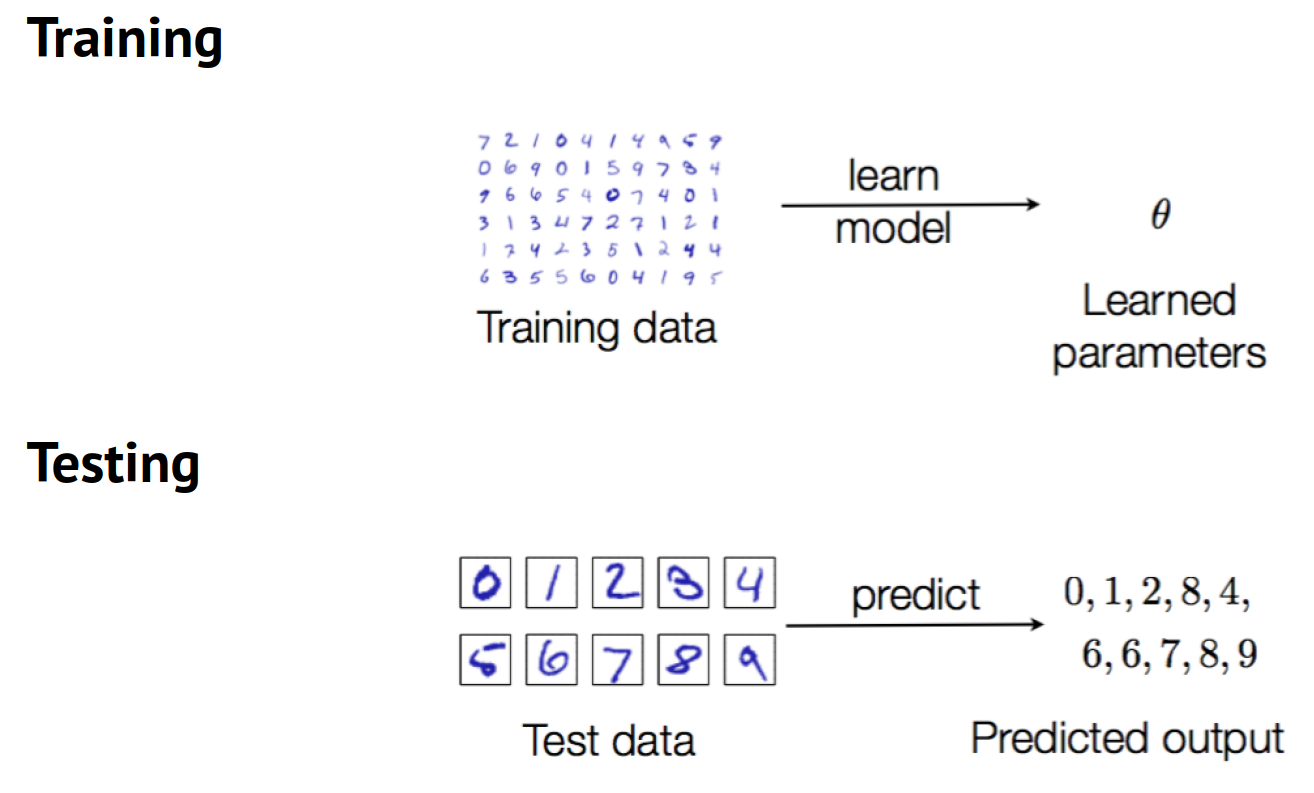
\includegraphics[scale=0.25]{01_intro_ml/02_img/general_paradigm}
	\end{figure}
\end{frame}


% Section: Problem Types in Machine Learning
%______________________________________________________________________
\section{Problem Types in Machine Learning}
\makedivider{Problem Types in Machine Learning}

% Subsection: Type of Training Information
% --------------------------------------------------------------------------------------------------------
\subsection{Type of Training Information}

% Type of Training Information
\begin{frame}{Type of Training Information}{}
	\begin{itemize}
		\item \highlight{Supervised learning}
		\begin{itemize}
			\item `Teacher' provides \textbf{gold labels}
			\item E.\,g. neural networks, decision trees, linear regression
		\end{itemize}
		\item \highlight{Unsupervised learning}
		\begin{itemize}
			\item Labels are \textbf{not} known during training
			\item E.\,g. clustering, density estimation, association rule mining
		\end{itemize}
		\item \highlight{Reinforcement learning}
		\begin{itemize}
			\item Environment provides rewards for actions but correct action is unknown
			\item E.\,g. policy-iteration, Q-learning, SARSA
		\end{itemize}
		\item \highlight{Semi-supervised learning} (partly labeled data)
	\end{itemize}
\end{frame}


% Type of Training Information (Ctd.)
\begin{frame}{Type of Training Information (Ctd.)}{}
	\begin{figure}
	\centering
	\begin{tikzpicture}[
		scale=0.5,
		every node/.style={scale=0.8},
		block/.style={
			draw=black,
			thick,
			align=left
		},
		arrow/.style={
			shorten >=0.2cm,
			shorten <=0.2cm,
			->,
			thick
		}
	]
	
		\node[block] (A) at (0,4) {
			\textbf{Supervised Learning} \\
			$\bullet$ A `teacher' provides gold labels \\
			$\bullet$ Neural networks, decision trees, linear regression
		};

		\node[block] (B) at (-5,0) {
			\textbf{Reinforcement Learning} \\
			$\bullet$ Feedback only \\
			$\bullet$ No labels
		};

		\node[block] (C) at (5,0) {
			\textbf{Semi-Supervised Learning} \\
			$\bullet$ Partly labeled data
		};

		\node[block] (D) at (0,-4) {
			\textbf{Unsupervised Learning} \\
			$\bullet$ No labels available \\
			$\bullet$ Clustering, Apriori, ...
		};
	
		\draw[arrow] (A) -- (B);
		\draw[arrow] (A) -- (C);
		\draw[arrow] (B) -- (D);
		\draw[arrow] (C) -- (D);

	\end{tikzpicture}
\end{figure}
\end{frame}


% Supervised Learning
\begin{frame}{Supervised Learning}{}
	\divideTwo{0.49}{
		\begin{itemize}
			\small
			\item A single row is called \highlight{example}
			\item An example without class label is called \highlight{instance}
			\item \highlight{Predictors:}
			\begin{itemize}
				\scriptsize
				\item \texttt{Outlook} $\in \{sunny, overcast, rainy\}$
				\item \texttt{Temperature} $\in \{hot, mild, cool\}$
				\item \texttt{Humidity} $\in \{high, normal\}$
				\item \texttt{Wind} $\in \{weak, strong\}$
			\end{itemize}
			\item \highlight{Label:}
			\begin{itemize}
				\scriptsize
				\item \texttt{PlayGolf} $\in \{yes, no\}$
				\item Given a new instance, we want to predict its label
			\end{itemize}
			\item \textbf{Label for the new instance???}
		\end{itemize}
	}{0.49}{
		\vspace*{2mm}
		\begin{table}
	\scalebox{0.6}{
	\begin{tabular}{| c | c | c | c || c |}
		\hline
		\highlight{Outlook} 		&
		\highlight{Temperature} 	&
		\highlight{Humidity} 		&
		\highlight{Wind} 			&
		\highlight{PlayGolf}		\\ \hline\hline
		sunny 	& hot 			& high 		& weak 		& \textbf{no}		\\ \hline
		sunny 	& hot 			& high 		& strong 	& \textbf{no} 		\\ \hline
		overcast 	& hot 			& high 		& weak 		& \textbf{yes} 		\\ \hline
		rainy 	& mild 			& high 		& weak 		& \textbf{yes} 		\\ \hline
		rainy 	& cool 			& normal 	& weak 		& \textbf{yes} 		\\ \hline
		rainy 	& cool 			& normal 	& strong 	& \textbf{no} 		\\ \hline
		overcast 	& cool 			& normal 	& strong 	& \textbf{yes} 		\\ \hline
		sunny 	& mild 			& high 		& weak 		& \textbf{no} 		\\ \hline
		sunny 	& cool 			& normal 	& weak 		& \textbf{yes} 		\\ \hline
		rainy 	& mild 			& normal 	& weak 		& \textbf{yes}		\\ \hline
		sunny 	& mild 			& normal 	& strong 	& \textbf{yes} 		\\ \hline
		overcast 	& mild 			& high 		& strong 	& \textbf{yes} 		\\ \hline
		overcast 	& hot 			& normal 	& weak 		& \textbf{yes}		\\ \hline
		rainy 	& mild 			& high 		& strong 	& \textbf{no} 		\\ \hline\hline
		rainy 	& mild 			& normal	& strong		& \highlight{???}		\\ \hline
	\end{tabular}}
\end{table}
	}
\end{frame}


% Supervised Learning: General Approach
\begin{frame}{Supervised Learning: General Approach}{}
	\vspace*{-5mm}
	\begin{figure}
	\centering
	\begin{tikzpicture}[
		scale=1.0,
		block/.style={
			draw=black,
			minimum width={4cm}
		},
		arrow/.style={
			->,
			thick,
			style=double
		}
	]
	
		\node[block] (A) at (0,2) {\textbf{Training Set} $\bm{\mathcal{D}}$};
		\node[block] (B) at (0,0) {\textbf{Learning Algorithm}};
		\node[block,pattern=north west lines,pattern color=lightgray,align=center] (C) at (-5,-2)
			{\textbf{Input/} \\ \textbf{Features}};
		\node[block,align=center] (D) at (0,-2) {\highlight{Hypothesis $\bm{h}$,} \\ \highlight{Model}};
		\node[block,pattern=north west lines,pattern color=lightgray,align=center] (E) at (5,-2)
			{\textbf{Output/} \\ \textbf{Prediction}};

		\draw[arrow] (A) -- node[right] {put into} (B);
		\draw[arrow] (B) -- node[right] {yields} (D);
		\draw[arrow] (C) -- (D);
		\draw[arrow] (D) -- (E);

	\end{tikzpicture}
\end{figure}
\end{frame}


% Unsupervised Learning
\begin{frame}{Unsupervised Learning}{}
	\divideTwo{0.49}{
		\vspace*{5mm}
		\begin{figure}
	\centering
	\begin{tikzpicture}[
		scale=0.7
	]

		\begin{axis}[
			xlabel={$\bm{Feature_1}$},
			ylabel={$\bm{Feature_2}$},
			ticks=none,
			x=2cm,
			y=3cm
		]
	
			\addplot[
				only marks,mark=*,mark size=2.5,fill=myblue1
			] table{04_ml_introduction/05_data/data_moons.txt};
    		\end{axis}
	\end{tikzpicture}
\end{figure}
	}{0.49}{
		\begin{itemize}
			\item There are \textbf{no} labels
			\item Try to find regularities in the data
			\item Examples for unsupervised learning:
			\begin{itemize}
				\item \highlight{Clustering}
				\item \highlight{Density estimation}
				\item \highlight{Dimensionality reduction}
			\end{itemize}
		\end{itemize}
	}
\end{frame}


% Subsection: Availability of Training Examples
% --------------------------------------------------------------------------------------------------------
\subsection{Availability of Training Examples}

% Availability of Training Examples
\begin{frame}{Availability of Training Examples}{}
	\begin{itemize}
		\item \highlight{Batch Learning}
		\begin{itemize}
			\item The learner is provided with a fixed set of training examples
			\item Cf. weather data set
			\item E.\,g. neural networks, decision trees
		\end{itemize}
		\item \highlight{Incremental / Online Learning}
		\begin{itemize}
			\item Constant stream of training examples
			\item The model is updated as new training examples arrive
			\item E.\,g. k-nearest-neighbors
		\end{itemize}
		\item Active Learning (\textit{not covered})
	\end{itemize}
\end{frame}


% Subsection: Type of Target Variable
% --------------------------------------------------------------------------------------------------------
\subsection{Type of Target Variable}

% Type of Target Variable: Regression
\begin{frame}{Type of Target Variable: Regression}{}
	\divideTwo{0.49}{
		\highlight{Regression}
		\begin{itemize}
			\item Learn a mapping into a continuous space
			\begin{itemize}
				\item $\mathcal{O} = \mathbb{R}$
				\item $\mathcal{O} = \mathbb{R}^3$
			\end{itemize}
			\item E.\,g. curve fitting, financial analysis, housing prices, ...
		\end{itemize}
	}{0.49}{
		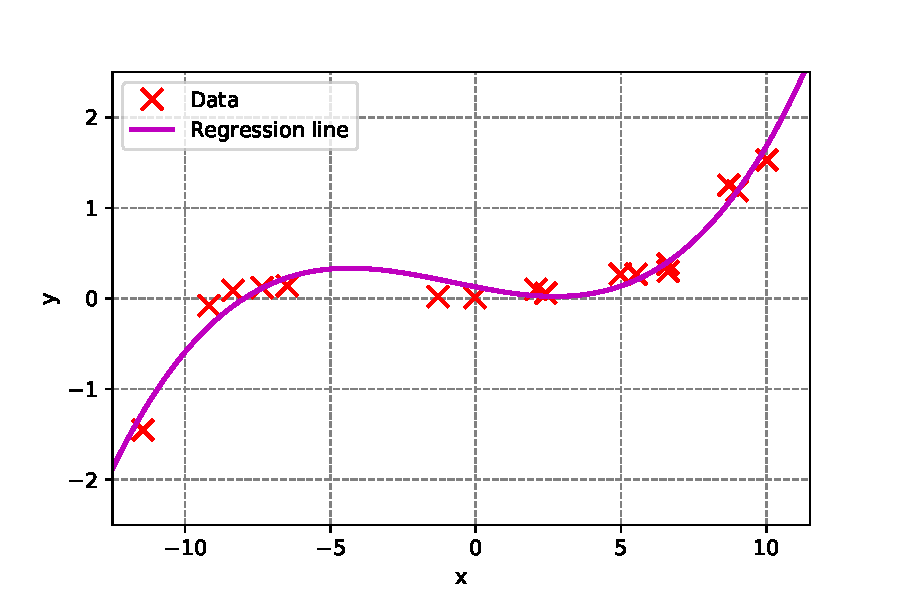
\includegraphics[scale=0.5]{01_intro_ml/02_img/regression_example}
	}
\end{frame}


% Type of Target Variable: Classification
\begin{frame}{Type of Target Variable: Classification}{}
	\divideTwo{0.49}{
		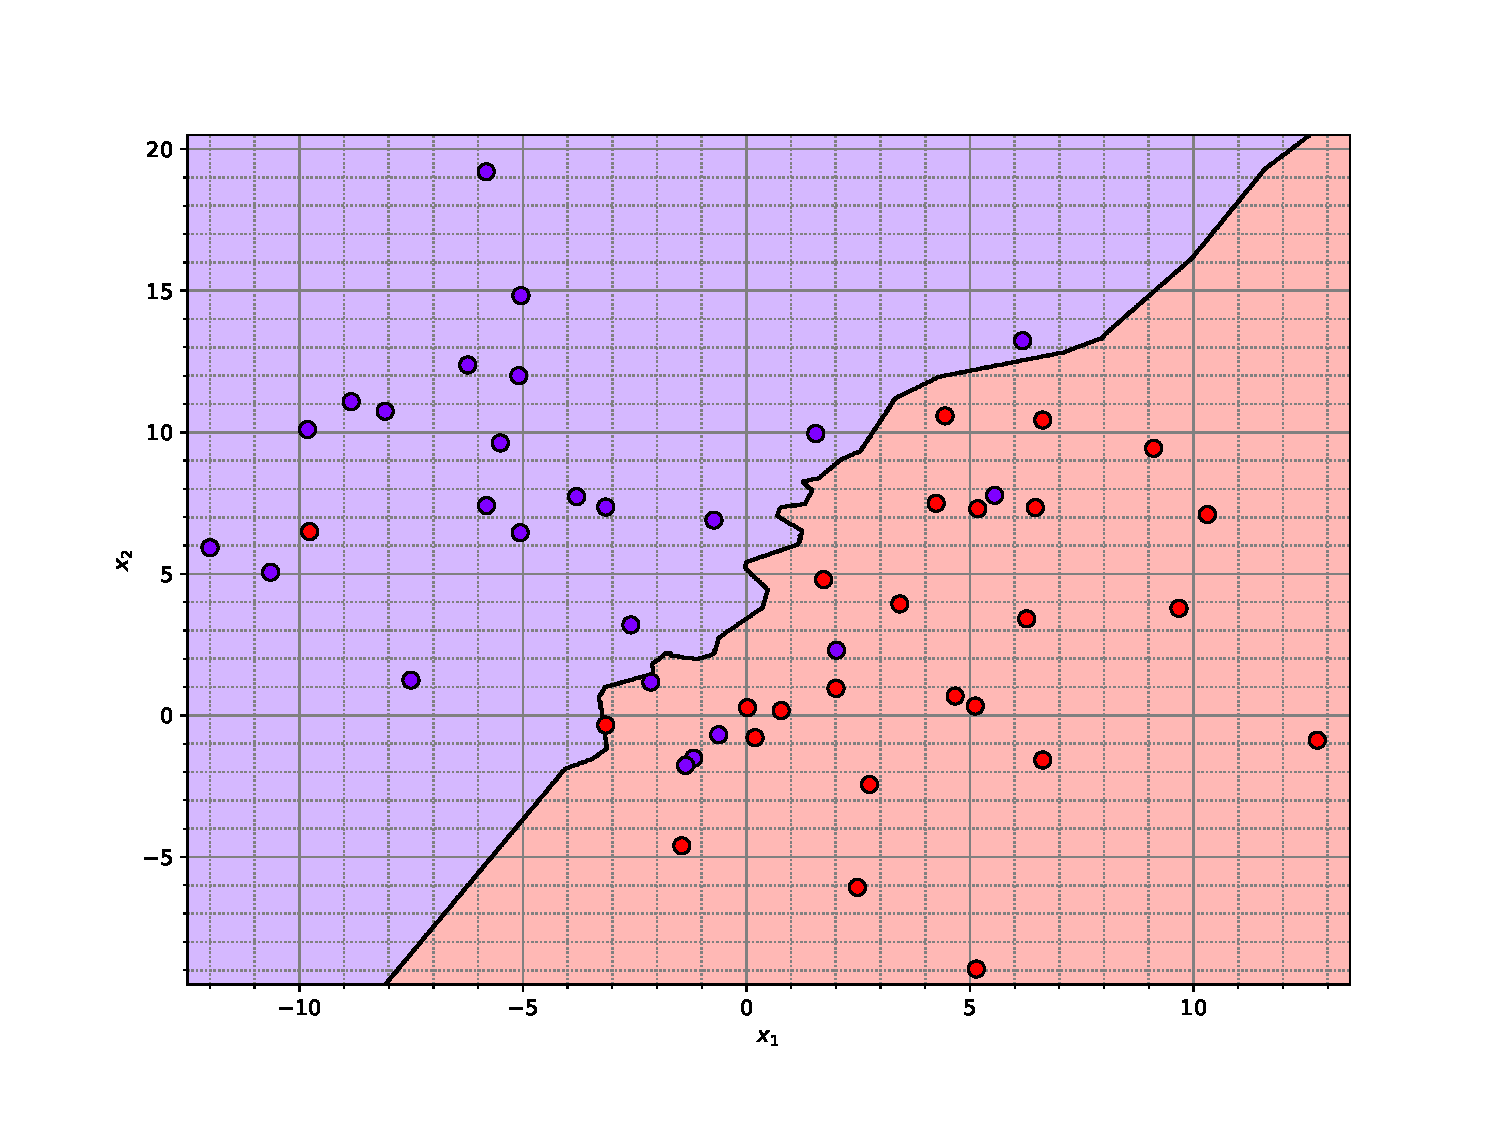
\includegraphics[scale=0.25]{01_intro_ml/02_img/classification_example}
	}{0.49}{
		\highlight{Classification}
		\begin{itemize}
			\item Learn a mapping into a discrete space, e.\,g.
			\begin{itemize}
				\item $\mathcal{O} = \{0, 1\}$ (binary classification)
				\item $\mathcal{O} = \{0, 1, 2, 3, ...\}$
				\item $\mathcal{O} = \{verb, noun, adverb, ...\}$
			\end{itemize}
			\item Examples:
			\begin{itemize}
				\item Spam / no spam
				\item Digit recognition
				\item Part of speech tagging
			\end{itemize}
		\end{itemize}
	}
\end{frame}


% Section: Key Challenges in Machine Learning
%______________________________________________________________________
\section{Key Challenges in Machine Learning}
\makedivider{Key Challenges in Machine Learning}

% Subsection: Generalization from Training Data
% --------------------------------------------------------------------------------------------------------
\subsection{Generalization from Training Data}

% Generalization from Training Data
\begin{frame}{Generalization from Training Data}{}\important
	\begin{itemize}
		\item Learning doest not mean memorizing the training data
		\item What if we see input that we \textbf{haven't seen before}?
		\item Example OCR (\textbf{O}ptical \textbf{C}haracter \textbf{R}ecognition):
		\begin{figure}
			\centering
			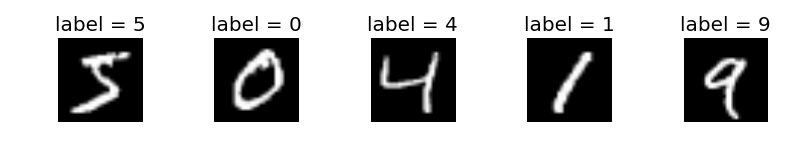
\includegraphics[scale=0.4]{01_intro_ml/02_img/mnist_digits}
		\end{figure}
		\vspace*{-4mm}
		\hfill{\scriptsize Hand-written digits from the MNIST data set}
		\begin{itemize}
			\item Predict the character given the input image
			\item \Highlight{People have different hand-writings}
		\end{itemize}
	\end{itemize}
\end{frame}


% Generalization from Training Data (Ctd.)
\begin{frame}{Generalization from Training Data (Ctd.)}{}\important
	\divideTwo{0.49}{
		\highlight{What is the problem here?}
		\begin{itemize}
			\item Complex decision boundary
			\item This leads to \Highlight{$\skull$ Overfitting $\skull$}
			\begin{itemize}
				\item The model is too expressive...
				\item ...and adapts to \textbf{idiosyncrasies} of the training data
			\end{itemize}
		\end{itemize}
	}{0.49}{
		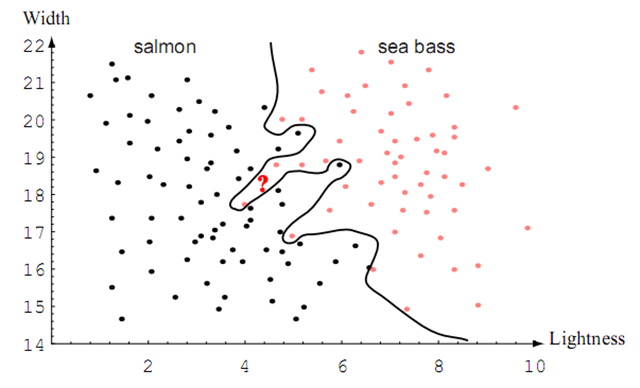
\includegraphics[scale=0.3]{01_intro_ml/02_img/salmon_sea_bass_overfitting}
	}
	\vspace*{2mm}
	\begin{boxBlueNoFrame}
		\textbf{Solution:} Choose a simpler model (cf. \textbf{Occam's razor})
	\end{boxBlueNoFrame}
\end{frame}


% Generalization from Training Data (Ctd.)
\begin{frame}{Generalization from Training Data (Ctd.)}{}\important
	\divideTwo{0.49}{
		\vspace*{1mm}
		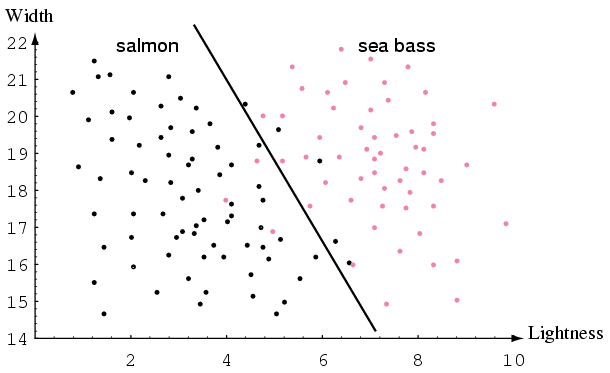
\includegraphics[scale=0.3]{01_intro_ml/02_img/salmon_sea_bass}
	}{0.49}{
		\begin{itemize}
			\item Linear (less complex) model
			\item Allow for \textbf{misclassifications} of some training examples
			\item \textbf{Better generalization} to unseen instances
		\end{itemize}
	}
\end{frame}


% A Prominent Example of Overfitting
\begin{frame}{A Prominent Example of Overfitting}{}
	\begin{figure}
		\centering
		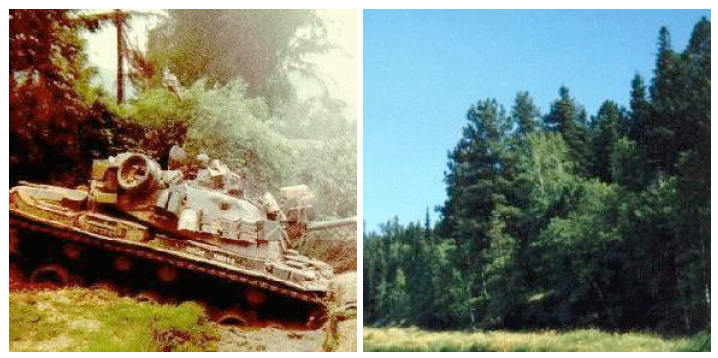
\includegraphics[scale=0.5]{01_intro_ml/02_img/tanks_overfitting}
	\end{figure}
\end{frame}


% Subsection: Feature Selection / Feature Engineering
% --------------------------------------------------------------------------------------------------------
\subsection{Feature Selection / Feature Engineering}

% Choosing the right Features
\begin{frame}{Choosing the right Features}{}
	\highlight{When stuck, move to a different perspective!}
	\vspace*{-2mm}
	\begin{figure}
	\centering
	\begin{tikzpicture}[
		scale=0.6
	]
		
		\node[align=center] at (-10,0) {$\mathcal{X}$ \\ \tiny Input space};
		\node (X) at (-5,0) {
			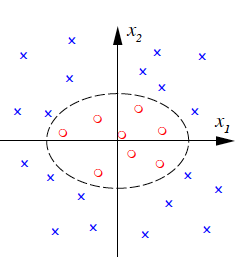
\includegraphics[scale=0.5]{01_intro_ml/02_img/input_space}
		};

		\node[align=center] at (10,0) {$\mathcal{F}$ \\ \tiny Feature space};
		\node (F) at (5,0) {
			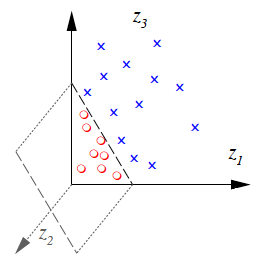
\includegraphics[scale=0.5]{01_intro_ml/02_img/feature_space}
		};

		\draw[->,ultra thick] (X) -- node[above] {$\phi : \mathcal{X} \mapsto \mathcal{F}$} (F);
		
	\end{tikzpicture}
\end{figure}
	\vspace*{-2mm}
	\begin{equation*}
		\phi(x_1, x_2) \mapsto \left( x_1^2, \sqrt{2} x_1 x_2, x_2^2 \right) = (z_1, z_2, z_3)
	\end{equation*}
\end{frame}


% Curse of Dimensionality
\begin{frame}{Choosing the right Features}{}
	\highlight{But: Beware of the \highlight{curse of dimensionality}!}
	
	\begin{figure}
		\divideTwo{0.59}{
			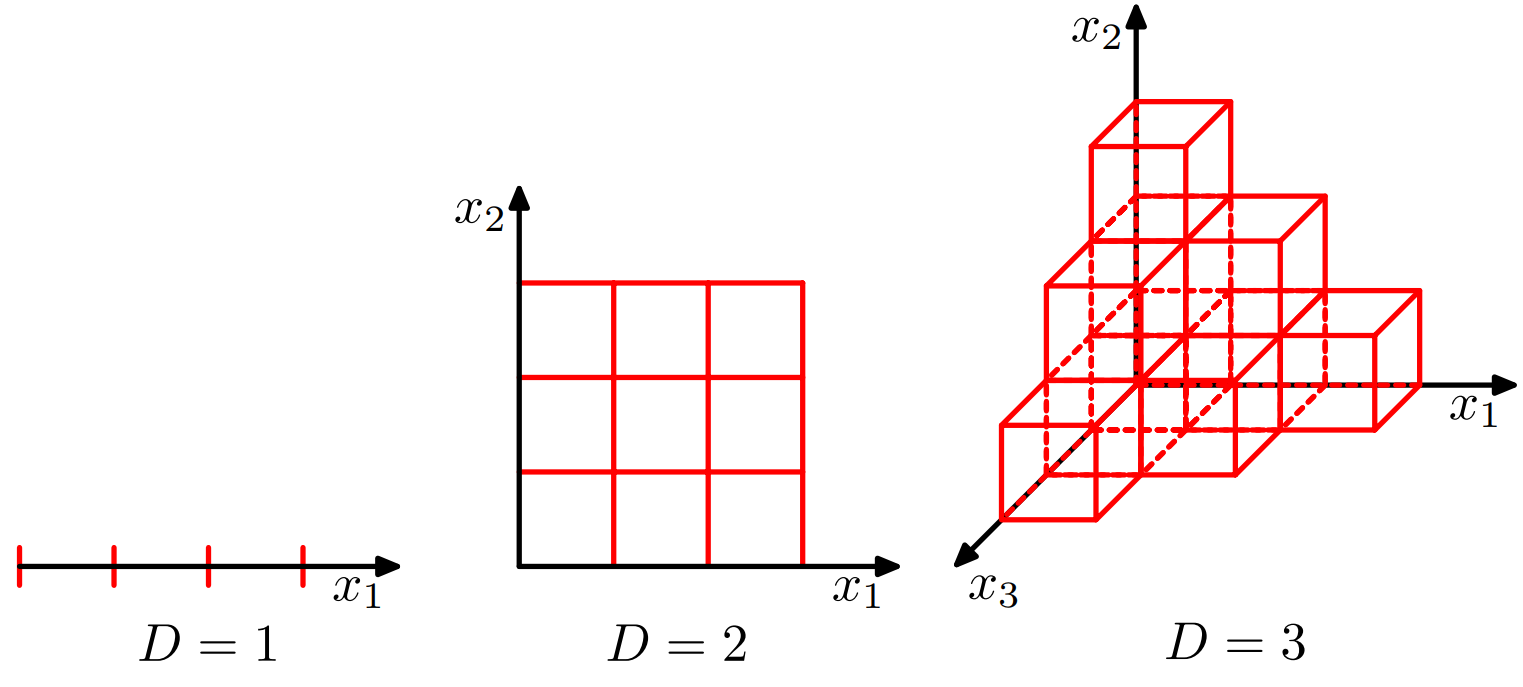
\includegraphics[scale=0.2]{01_intro_ml/02_img/curse_of_dimensionality}
		}{0.39}{
			\begin{itemize}
				\item Too many features significantly \textbf{slow down} the ML algorithm
				\item Need \textbf{exponential} amount of training data
				\item Dimensionality reduction
			\end{itemize}
		}
	\end{figure}
	\citeAuthor{Image taken from}{Bishop.2006}{p.\,35}
\end{frame}


% Subsection: Performance Measurement
% --------------------------------------------------------------------------------------------------------
\subsection{Performance Measurement}

% Performance Measurement
\begin{frame}{Performance Measurement}{}
	\begin{itemize}
		\item How do we measure performance?
		\begin{itemize}
			\item 99\,\% correct classification in speech recognition: What does it really mean?
			\item \textit{We understand the meaning of the sentence?}, \textit{We understand every word?},
				\textit{For all speakers?}
		\end{itemize}
		\item We need more \textbf{concrete numbers}:
		\begin{itemize}
			\item \% of correctly classified letters
			\item Average distance driven (until accident, ...)
			\item \% of games won
			\item \% of correctly recognized words, sentences, etc.
		\end{itemize}
		\item \Highlight{Training vs. testing performance}
	\end{itemize}
\end{frame}


% Training vs. Testing Performance
\begin{frame}{Training vs. Testing Performance}{}
	\divideTwo{0.49}{
		\begin{itemize}
			\item Evaluate on data which was \textbf{not used} for training {\footnotesize \highlight{(out-of-sample)}}
			\item Two-way split: \\
				\texttt{Train - Test}
			\item Even better: \\
				\texttt{Train - Dev - Test}
			\vspace{2mm}
			\begin{tabbing}
				\hspace*{1.5cm}\= \kill
				\textbf{Train:}	\>	Train model 			\\
				\textbf{Dev:} 	\>	Tune hyper-parameters 	\\
				\textbf{Test:} 	\>	Test final model
			\end{tabbing}
		\end{itemize}
	}{0.49}{
		\centering
		
\includegraphics[scale=0.4]{01_intro_ml/02_img/train_test_split_meme}
	}
\end{frame}


% Performance Measurement (Ctd.)
\begin{frame}{Performance Measurement (Ctd.)}{}
	\begin{itemize}
		\item We also need to define the right \highlight{error metric}:
	\end{itemize}
	\begin{figure}
		\centering
		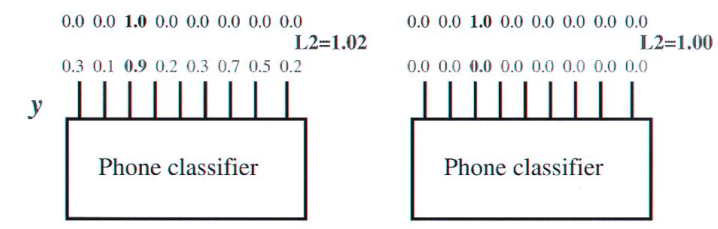
\includegraphics[scale=0.5]{01_intro_ml/02_img/error_metric}
	\end{figure}
	\vspace*{-4mm}
	\begin{itemize}
		\item Which is better?
		\item Euclidean distance (L2-norm) might be useless
	\end{itemize}
\end{frame}


% Subsection: Model Selection
% --------------------------------------------------------------------------------------------------------
\subsection{Model Selection}

% Model Selection
\begin{frame}{Model Selection}{}
	\begin{itemize}
		\item What is the \textbf{right model}?
		\item The learned parameters (here: $\bm{w}$) can mean a lot of different things:
	\end{itemize}
	
	\begin{figure}
		\divideTwo{0.49}{
			\footnotesize
			\begin{itemize}
				\item May characterize a family of functions
				\item May be parameters of a probability distribution
				\item $\bm{w}$ may be a vector, adjacency matrix, graph, ...
			\end{itemize}
		}{0.49}{
			\begin{figure}
				\centering
				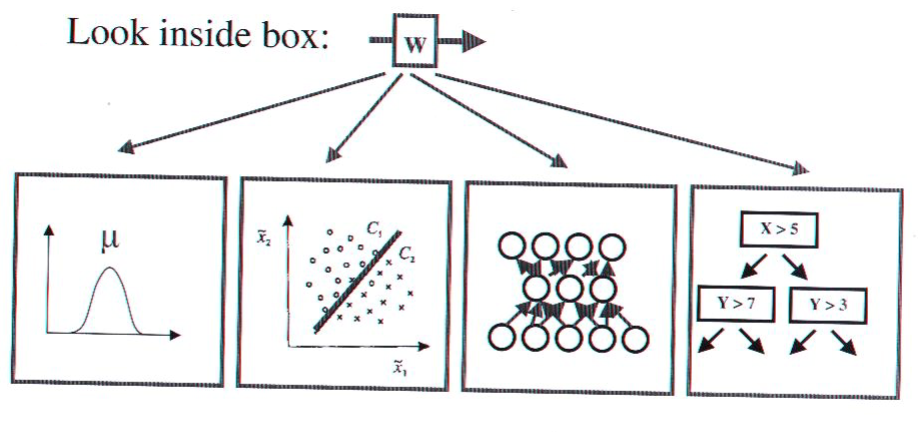
\includegraphics[scale=0.25]{01_intro_ml/02_img/model_selection}
			\end{figure}
		}
	\end{figure}
\end{frame}


% Subsection: Computation
% --------------------------------------------------------------------------------------------------------
\subsection{Computation}

% Computation
\begin{frame}{Computation}{}
	Even if the other problems are solved, \Highlight{computation is usually quite hard}:
	\begin{itemize}
		\item Learning involves optimization of parameters
		\item Find / Search for best model parameters
		\begin{itemize}
			\item GoogleNet has $\approx$ 6.5 million parameters
			\item Often GPUs (\textbf{G}raphics \textbf{P}rocessing \textbf{U}nit) are needed
			\item Google invented TPUs (\textbf{T}ensor \textbf{P}rocessing \textbf{U}nit)
		\end{itemize}
		\item Often we have to deal with thousands, millions, ... of training examples
		\item Given a model, the prediction has to be computed efficiently
	\end{itemize}
\end{frame}


% Section: Machine Learning Applications
%______________________________________________________________________
\section{Machine Learning Applications}
\makedivider{Machine Learning Applications}

% Subsection: Natural Language Processing
% --------------------------------------------------------------------------------------------------------
\subsection{Natural Language Processing}

% Natural Language Processing
\begin{frame}{Applications in Natural Language Processing}{}
	\begin{itemize}
		\item \textbf{E-mail filtering:}
		\begin{figure}
			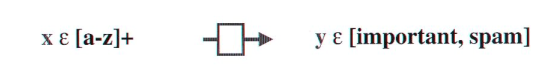
\includegraphics[scale=0.5]{01_intro_ml/02_img/email_filtering}
		\end{figure}
		\item \textbf{Speech Recognition:}
		\begin{figure}
			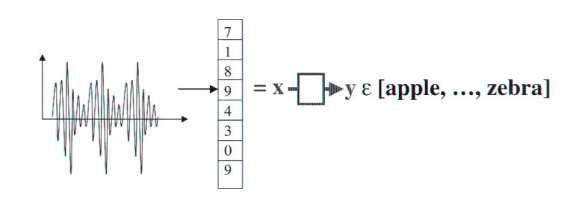
\includegraphics[scale=0.5]{01_intro_ml/02_img/speech_recognition}
		\end{figure}
	\end{itemize}
\end{frame}


% Subsection: Computer Vision
% --------------------------------------------------------------------------------------------------------
\subsection{Computer Vision}

% Applications in Computer Vision
\begin{frame}{Applications in Computer Vision}{}
	\divideTwoTop{0.49}{
		\textbf{Face detection:}
		\begin{figure}
			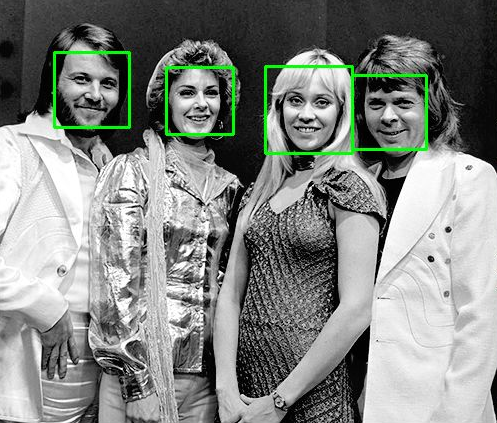
\includegraphics[scale=0.35]{01_intro_ml/02_img/face_detection}
		\end{figure}
	}{0.49}{
		\textbf{Traffic sign detection:}
		\begin{figure}
			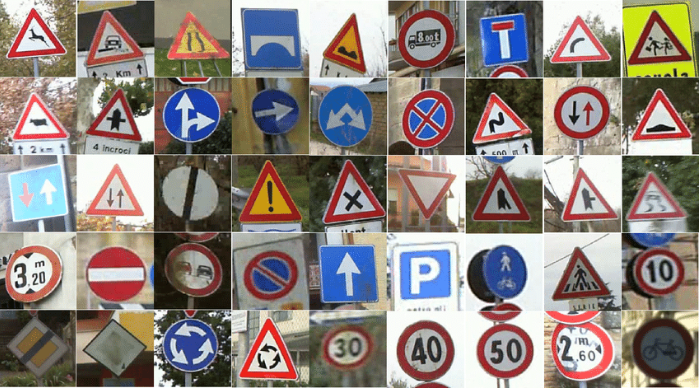
\includegraphics[scale=0.3]{01_intro_ml/02_img/traffic_sign_detection}
		\end{figure}
	}
\end{frame}


% Applications in Computer Vision (Ctd.)
\begin{frame}{Applications in Computer Vision (Ctd.)}{}
	\textbf{Optical character recognition:}
	\begin{figure}
		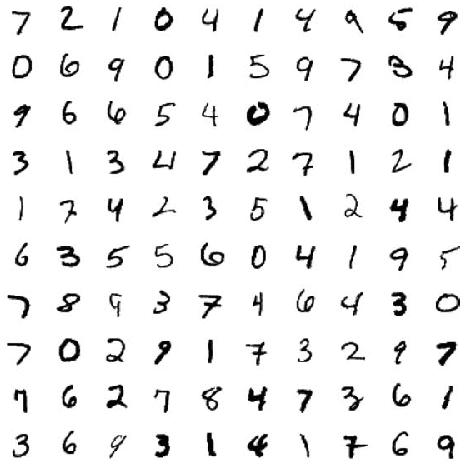
\includegraphics[scale=0.3]{01_intro_ml/02_img/digit_recognition}
	\end{figure}
	{\footnotesize See \href{https://www.youtube.com/watch?v=yxuRnBEczUU}{\linkstyle{Demonstration LeNet}}}
\end{frame}


% Subsection: Robotics
% --------------------------------------------------------------------------------------------------------
\subsection{Robotics}

% Applications in Robotics
\begin{frame}{Applications in Robotics}{}
	\divideTwoTop{0.49}{
		\textbf{Robot control:}
		\vspace*{0.8mm}
		\begin{figure}
			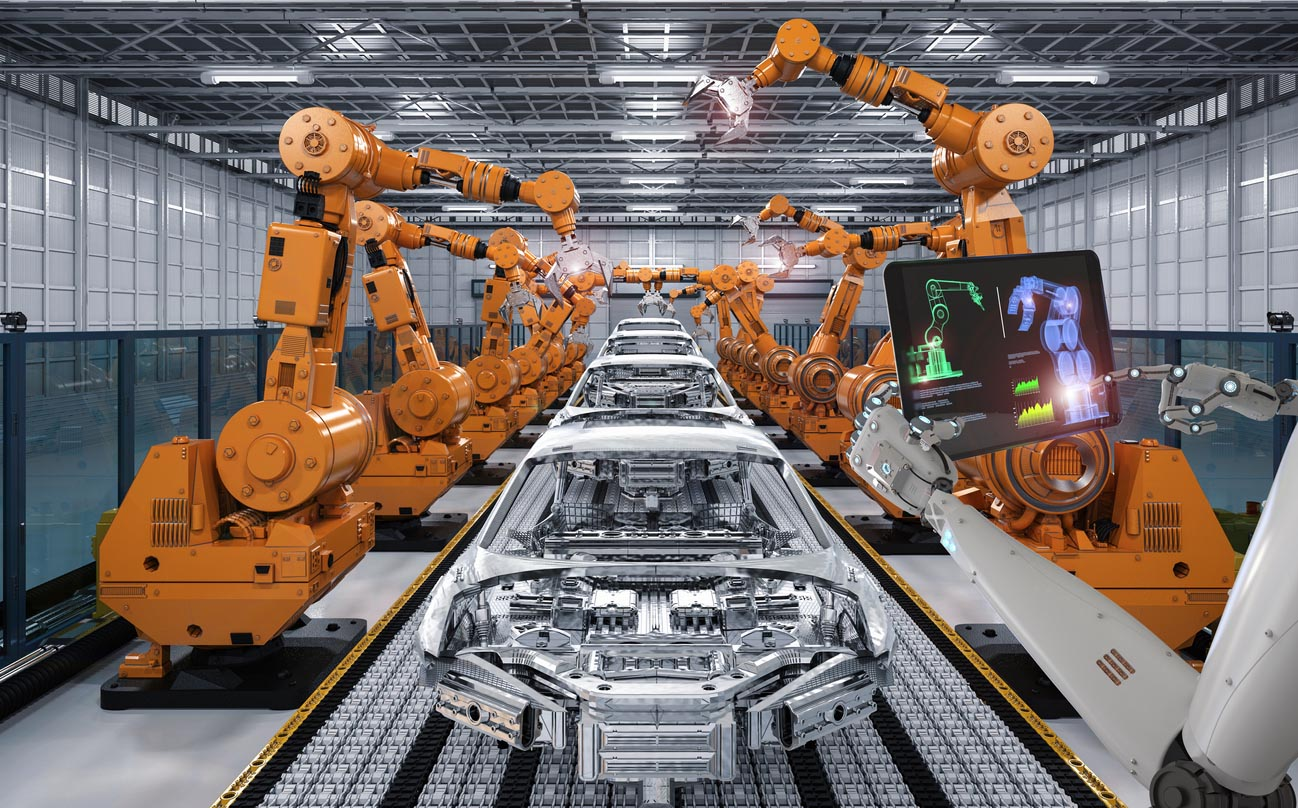
\includegraphics[scale=0.1125]{01_intro_ml/02_img/robot_control}
		\end{figure}
	}{0.49}{
		\textbf{Autonomous driving:}
		\begin{figure}
			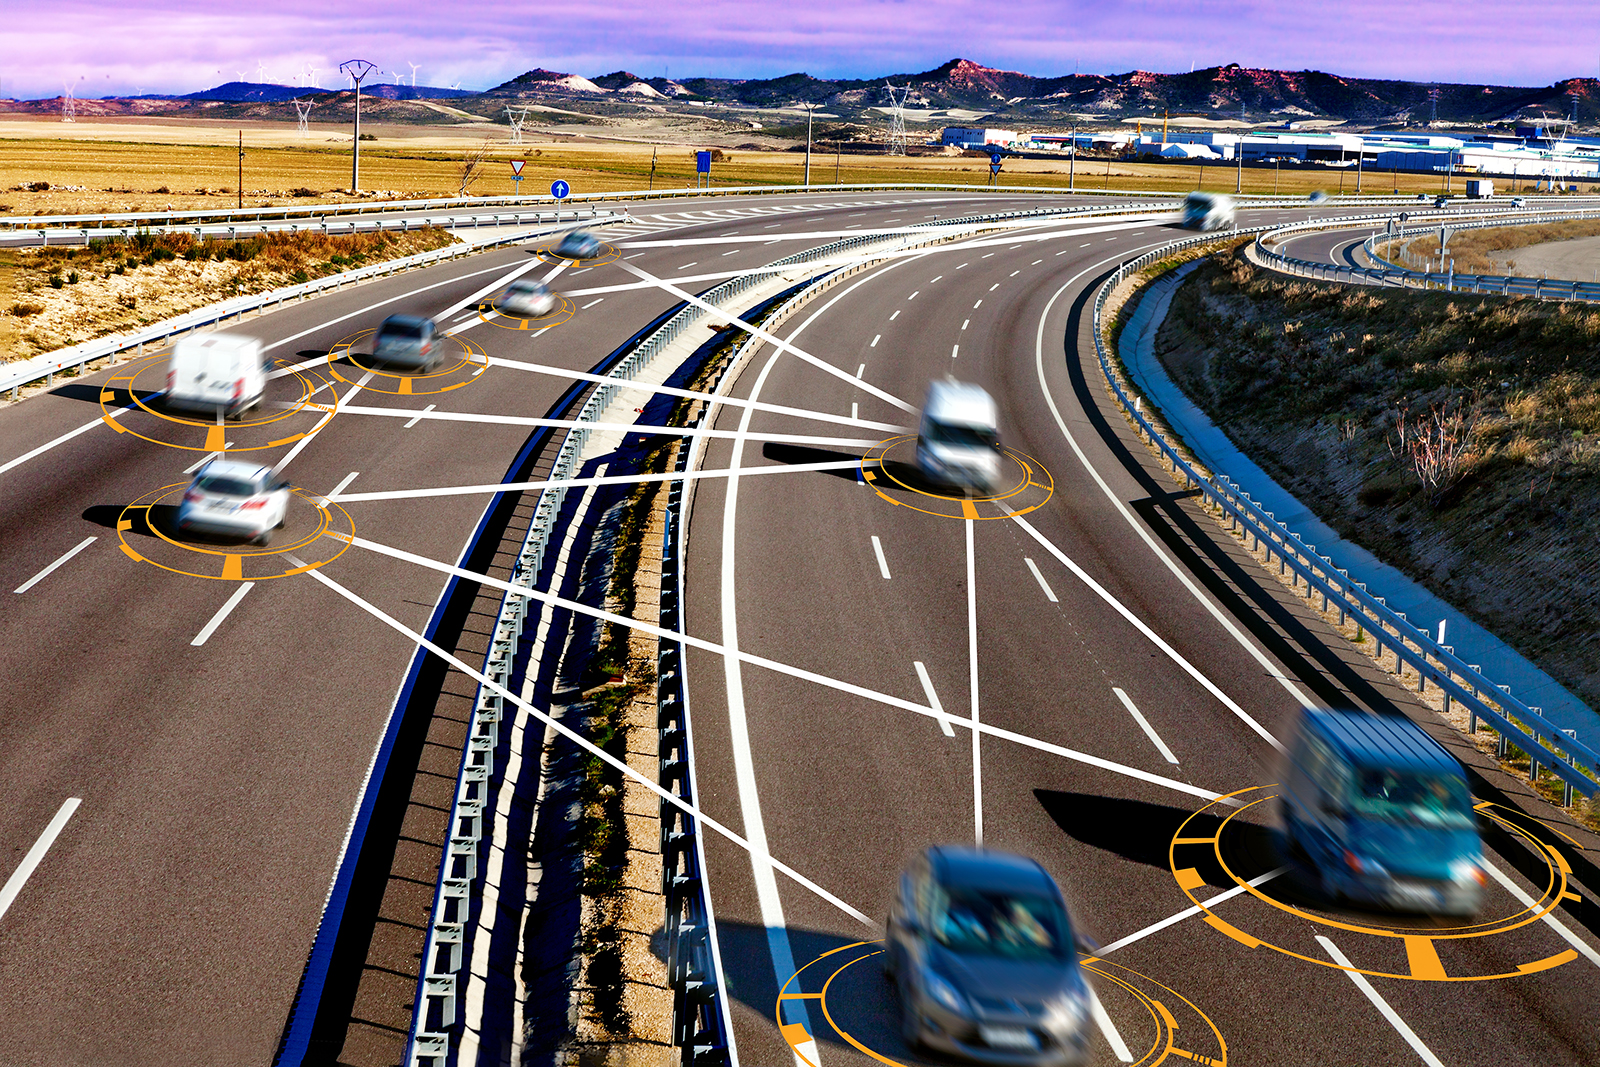
\includegraphics[scale=0.35]{01_intro_ml/02_img/autonomous_driving}
		\end{figure}
	}
\end{frame}


% Why Machine Learning?
\begin{frame}{Why Machine Learning?}{}
	\begin{figure}
		\centering
		
\includegraphics[scale=0.4]{01_intro_ml/02_img/why_machine_learning}
	\end{figure}
\end{frame}


% Section: Wrap-Up
%______________________________________________________________________
\section{Wrap-Up}
\makedivider{Wrap-Up}

% Subsection: Summary
% --------------------------------------------------------------------------------------------------------
\subsection{Summary}

% Summary
\begin{frame}{Summary}{}
	\begin{itemize}
		\item Vast amounts of data are prohibitive for manual inspection
		\item Machine learning algorithms learn \textbf{without being explicitly programmed}
		\item \textbf{Important distinctions:}
		\begin{itemize}
			\item Supervised learning $\Leftrightarrow$ unsupervised learning
			\item Classification $\Leftrightarrow$ regression
		\end{itemize}
		\item \textbf{Challenges:}
		\begin{enumerate}
			\item Generalization
			\item Feature engineering
			\item Performance measurement
			\item Model selection
			\item Computation
		\end{enumerate}
	\end{itemize}
\end{frame}


% Subsection: Self-Test Questions
% --------------------------------------------------------------------------------------------------------
\subsection{Self-Test Questions}

% Self-Test Questions
\begin{frame}{Self-Test Questions}{}\important
	\begin{enumerate}
		\item What is the difference between supervised and unsupervised learning?
		\item What is regression?
		\item What does generalization mean?
		\item \textit{'The more features the better.'} Is this statement correct or not? Give reasons for your answer.
		\item Why do we need \texttt{train}, \texttt{dev} and \texttt{test} sets?
		\item True or false: 100\,\% train accuracy is desirable.
		\item State some applications of machine learning.
	\end{enumerate}
\end{frame}


% Subsection: Lecture Outlook
% --------------------------------------------------------------------------------------------------------
\subsection{Lecture Outlook}

\begin{frame}{What's next...?}{}
	\makeoverview{2}
\end{frame}


% Subsection: Recommended Literature and further Reading
% --------------------------------------------------------------------------------------------------------
\subsection{Recommended Literature and further Reading}

% Literature
%______________________________________________________________________
\begin{frame}{Recommended Literature and further Reading}{}
	\footnotesize
	\begin{thebibliography}{2}
		\literature{book}{Mitchell.1997}{[1] Machine Learning}
			{Tom Mitchell. McGraw-Hill Science. 1997.}{$\rightarrow$ \href{
				https://www.cs.ubbcluj.ro/~gabis/ml/ml-books/McGrawHill\%20-\%20Machine\%20Learning\%20-Tom\%20Mitchell.pdf
			}{\linkstyle{Link}}, cf. chapter 1 \textit{'Introduction'}}

		\literature{book}{Bishop.2006}{[2] Pattern Recognition and Machine Learning}
			{Christopher Bishop. Springer. 2006.}{$\rightarrow$ \href{
				http://users.isr.ist.utl.pt/~wurmd/Livros/school/Bishop\%20-\%20Pattern\%20Recognition\%20And\%20Machine\%20Learning\%20-\%20Springer\%20\%202006.pdf
			}{\linkstyle{Link}}, cf. chapter 1 \textit{'Introduction'}}
	\end{thebibliography}
\end{frame}


% Thank you
%______________________________________________________________________
\makethanks

\end{document}